% !TeX program = xelatex
\ifdefined\BookMaster\else
\documentclass[11pt,oneside]{article}
% !TeX program = xelatex
\usepackage[b5paper,left=22mm,right=22mm,top=20mm,bottom=22mm,footskip=11mm]{geometry}
\usepackage{fontspec}
\setmainfont{TeX Gyre Termes}
\setsansfont{TeX Gyre Heros}
\usepackage{amsmath,amssymb,mathtools,amsthm}
\renewcommand{\cdots}{\mathinner{\cdotp\cdotp\cdotp}}
\usepackage{graphicx,adjustbox,array,booktabs,longtable,multirow,enumitem,changepage,needspace}
\usepackage[table]{xcolor}
\usepackage{fancyhdr}
\raggedbottom
\interfootnotelinepenalty=10000
\newcommand{\BookFootnote}[2]{\begingroup\renewcommand{\thefootnote}{\fnsymbol{footnote}}\footnote[#1]{#2}\endgroup}
\newcommand{\BookFootnoteMark}[1]{\begingroup\renewcommand{\thefootnote}{\fnsymbol{footnote}}\footnotemark[#1]\endgroup}
\newcommand{\BookFootnoteText}[2]{\begingroup\renewcommand{\thefootnote}{\fnsymbol{footnote}}\footnotetext[#1]{#2}\endgroup}
\newenvironment{BookFloat}[1]{\par\addvspace{.6\baselineskip}\noindent\def\BookFloatID{#1}\begin{minipage}{\linewidth}\phantomsection\label{bookfloat:#1:start}}{\phantomsection\label{bookfloat:\BookFloatID:end}\end{minipage}\par\addvspace{.6\baselineskip}}

\usepackage[unicode,hidelinks]{hyperref}
\pagestyle{fancy}
\fancyhf{}
\newcommand{\BookFooter}{}
\fancyfoot[L]{\parbox[b]{\dimexpr\textwidth-15mm}{\footnotesize\BookFooter}}
\fancyfoot[R]{\footnotesize\thepage}
\renewcommand{\headrulewidth}{0pt}
\renewcommand{\footrulewidth}{0pt}
\setlength{\parindent}{0pt}
\setlength{\parskip}{0.2em}
\setlength{\emergencystretch}{3em}
\setlist{nosep,leftmargin=1.7em,labelsep=.65em}
\newif\ifBookNarrative
\BookNarrativetrue
\newenvironment{BookBody}{\setlength{\parindent}{0pt}}{}
\newcommand{\BookStatement}[1]{\par\addvspace{.6\baselineskip}\noindent #1\enspace\ignorespaces}
\newcommand{\BookLabel}[1]{\par\addvspace{.6\baselineskip}\needspace{3\baselineskip}\noindent\textbf{#1}\quad\ignorespaces}
\newcommand{\BookHeading}[1]{\par\addvspace{\baselineskip}\needspace{4\baselineskip}\noindent{\large\bfseries #1}\par\medskip}
\newcommand{\BookSubheading}[1]{\par\addvspace{.7\baselineskip}\needspace{3\baselineskip}\noindent{\bfseries #1}\par\smallskip}
\newcommand{\BookTextHeading}[1]{\par\addvspace{.7\baselineskip}\needspace{3\baselineskip}\noindent #1\par\smallskip}
\newcommand{\BookSectionTitle}[2]{\par\addvspace{1.2\baselineskip}\needspace{5\baselineskip}\noindent\colorbox{gray!25}{\sffamily\bfseries\small SECTION #1}\quad{\large\bfseries #2}\par\medskip}
\newcommand{\BookExerciseTitle}[1]{\par\addvspace{\baselineskip}\needspace{4\baselineskip}\noindent{\color{gray}\rule{1.5mm}{1.5mm}}\enspace{\large\bfseries Exercises #1}\par\medskip}
\newcommand{\BookBullet}[1]{\begin{list}{\textbullet}{\setlength{\leftmargin}{1.7em}\setlength{\labelwidth}{1em}\setlength{\labelsep}{.7em}\setlength{\topsep}{0pt}\setlength{\parsep}{0pt}\setlength{\itemsep}{0pt}}\item #1\end{list}}
\newcommand{\BookExercise}[2]{\begin{list}{\textbf{#1}}{\setlength{\leftmargin}{2.2em}\setlength{\labelwidth}{1.5em}\setlength{\labelsep}{.7em}\setlength{\topsep}{.15em}\setlength{\parsep}{0pt}\setlength{\itemsep}{0pt}}\item #2\end{list}}
\newcommand{\BookEnd}[1]{\unskip\nobreak\hfill\ensuremath{#1}}
\newcommand{\BookSource}[2]{\phantomsection\label{sourcepage:#1}} % Source-page anchors, retained through reflow.
\usepackage{multicol}
\usepackage{tikz}
\newcommand{\BookPartEntry}[2]{\par\noindent\makebox[17mm][l]{\bfseries Section #1}#2\par}
\newcommand{\BookPartTitle}[3]{\par\bigskip\noindent\begin{tikzpicture}\node[anchor=north west,inner sep=0pt,outer sep=0pt] (bookpart) at (0,0) {\begin{minipage}{\dimexpr\linewidth-.5pt}\hspace*{26mm}\begin{minipage}[t]{\dimexpr\linewidth-26mm}\begin{adjustbox}{max width=\linewidth}{\fontsize{20}{24}\selectfont\bfseries #2}\end{adjustbox}\par\vspace{6mm}\hrule\vspace{6mm}{\sffamily\footnotesize\setlength{\parskip}{.3em}#3}\vspace{3mm}\end{minipage}\end{minipage}};\path[shade,top color=gray!60,bottom color=white] (0,0) rectangle ([xshift=24mm]bookpart.south west);\node[anchor=north,font=\sffamily\bfseries\small] at (12mm,-2mm) {PART};\node[anchor=north,font=\sffamily\bfseries\Huge] at (12mm,-7mm) {#1};\end{tikzpicture}\par\bigskip}
\newsavebox{\BookMathBox}
\makeatletter
\newcommand{\BookInline}[1]{\leavevmode\hskip0pt\relax\begingroup\in@{\begin}{#1}\ifin@\sbox{\BookMathBox}{\(#1\)}\ifdim\wd\BookMathBox>\dimexpr\linewidth-1em\relax\resizebox{\dimexpr\linewidth-1em\relax}{!}{\usebox{\BookMathBox}}\else\(#1\)\fi\else\in@{\left}{#1}\ifin@\sbox{\BookMathBox}{\(#1\)}\ifdim\wd\BookMathBox>\dimexpr\linewidth-1em\relax\resizebox{\dimexpr\linewidth-1em\relax}{!}{\usebox{\BookMathBox}}\else\(#1\)\fi\else\(#1\)\fi\fi\endgroup\hskip0pt\relax}
\makeatother
\DeclareMathOperator{\Aut}{Aut}
\DeclareMathOperator{\End}{End}
\DeclareMathOperator{\Hom}{Hom}
\DeclareMathOperator{\GF}{GF}
\DeclareMathOperator{\irr}{irr}
\DeclareMathOperator{\lt}{lt}
\DeclareMathOperator{\lp}{lp}
\providecommand{\textcircled}[1]{\textnormal{(#1)}}

\begin{document}
\fi
\renewcommand{\BookFooter}{Section 5 Subgroups}
\pdfbookmark[0]{Section 5 Subgroups}{05_subgroups}
\ifdefined\BookMaster\else\setcounter{page}{52}\fi
% Source PDF page 69; original printed page 52
\BookSource{69}{52}
\BookNarrativetrue

\begin{BookBody}

\BookSectionTitle{5}{Subgroups}

\BookTextHeading{\textbf{Subsets and Subgroups}  }

\noindent You may have noticed that we sometimes have had groups contained within larger groups. For example, the group \BookInline{\mathbb{Z}} under addition is contained within the group \BookInline{\mathbb{Q}} under addition, which in turn is contained in the group \BookInline{\mathbb{R}} under addition. When we view the group \BookInline{\langle \mathbb{Z},\allowbreak + \rangle } as contained in the group \BookInline{\langle \mathbb{R},\allowbreak + \rangle,\allowbreak } it is very important to notice that the operation \BookInline{+ } on integers \BookInline{n} and \BookInline{m} as elements of \BookInline{\langle \mathbb{Z},\allowbreak + \rangle } produces the same element \BookInline{n+ m} as would result if you were to think of \BookInline{n} and \BookInline{m} as elements in \BookInline{\langle \mathbb{R},\allowbreak + \rangle.} Thus we should \textit{not} regard the group \BookInline{\langle \mathbb{Q}^{+ },\allowbreak \cdot \rangle } as contained in \BookInline{\langle \mathbb{R},\allowbreak + \rangle,\allowbreak } even though \BookInline{\mathbb{Q}^{+ }} is contained in \BookInline{\mathbb{R}} as a set. In this instance\BookInline{,\allowbreak 2\cdot 3= 6} in \BookInline{\langle \mathbb{Q}^{+ },\allowbreak \cdot \rangle,\allowbreak } while \BookInline{2+ 3= 5} in \BookInline{\langle \mathbb{R},\allowbreak + \rangle.} We are requiring not only that the set of one group be a subset of the set of the other, but also that the group operation on the subset be the\textit{ induced operation} that assigns the same element to each ordered pair from this subset as is assigned by the group operation on the whole set.

\BookLabel{5.1 Definition} If a subset \BookInline{H} of a group \BookInline{G} is closed under the binary operation of \BookInline{G} and if \BookInline{H} with the induced operation from \BookInline{G} is itself a group, then \BookInline{H} is a\textbf{ subgroup of} \BookInline{G.} We shall let \BookInline{H\leq G} or \BookInline{G\geq H} denote that \BookInline{H} is a subgroup of \BookInline{G,\allowbreak } and \BookInline{H<G} or \BookInline{G>H} shall mean \BookInline{H\leq G} but \BookInline{H\neq G.}\BookEnd{\blacksquare}

Thus \BookInline{\langle \mathbb{Z},\allowbreak + \rangle <\langle \mathbb{R},\allowbreak + \rangle } but \BookInline{\langle \mathbb{Q}^{+ },\allowbreak \cdot \rangle } is\textit{ not} a subgroup of \BookInline{\langle \mathbb{R},\allowbreak + \rangle,\allowbreak } even though as sets, \BookInline{\mathbb{Q}^{+ }\subset \mathbb{R}.} Every group \BookInline{G} has as subgroups \BookInline{G} itself and \BookInline{\{e\},\allowbreak } where \BookInline{e} is the identity element of \BookInline{G.}

\BookLabel{5.2 Definition} If \BookInline{G} is a group, then the subgroup consisting of \BookInline{G} itself is the\textbf{ improper subgroup} of \BookInline{G.} All other subgroups are\textbf{ proper subgroups}. The subgroup \BookInline{\{e\}} is the\textbf{ trivial subgroup} of \BookInline{G.} All other subgroups are\textbf{ nontrivial}\BookInline{.}\BookEnd{\blacksquare}

\noindent We turn to some illustrations.

\end{BookBody}

% Source PDF page 70; original printed page 53
\BookSource{70}{53}
\BookNarrativetrue

\begin{BookBody}

\BookLabel{5.3 Example} Let \BookInline{\mathbb{R}^{n}} be the additive group of all \BookInline{n-}component row vectors with real number entries. The subset consisting of all of these vectors having 0 as entry in the first component is a subgroup of \BookInline{\mathbb{R}^{n}.}\BookEnd{\blacktriangle}

\BookLabel{5.4 Example} \BookInline{\mathbb{Q}^{+ }} under multiplication is a proper subgroup of \BookInline{\mathbb{R}^{+ }} under multiplication. \BookEnd{\blacktriangle}

\BookLabel{5.5 Example} The \BookInline{n}\textbf{th} roots of unity in \BookInline{\mathbb{C},\allowbreak U_{n},\allowbreak } form a subgroup of \BookInline{U,\allowbreak } the complex numbers whose absolute value is 1, which in turn is a subgroup of \BookInline{\mathbb{C}^{\ast },\allowbreak } the nonzero complex numbers under multiplication\BookInline{.}\BookEnd{\blacktriangle}

\BookLabel{5.6 Example} Recall that \BookInline{S_{\mathbb{Z}_{n}}} is the set of all one-to-one functions mapping \BookInline{\mathbb{Z}_{n}} onto \BookInline{\mathbb{Z}_{n}} and \BookInline{D_{n}} is the set of all one-to-one functions \BookInline{\phi } mapping \BookInline{\mathbb{Z}_{n}} onto \BookInline{\mathbb{Z}_{n}} with the further property that the line segment between \BookInline{i} and \BookInline{j} is an edge of the regular \BookInline{n-}gon \BookInline{P_{n}} if and only if the line segment between \BookInline{\phi (i)} and \BookInline{\phi (j)} is an edge. \BookInline{D_{n}\subseteq S_{\mathbb{Z}_{n}}}. Since both \BookInline{D_{n}} and \BookInline{S_{\mathbb{Z}_{n}}} are groups under composition of functions, \BookInline{D_{n}\leq S_{\mathbb{Z}_{n}}} \BookInline{.}\BookEnd{\blacktriangle}

\BookLabel{5.7 Example} There are two different types of group structures of order 4 (see Exercise 20 of Section 2). We describe them by their group tables (Tables 5.8 and 5.9). The group \BookInline{V} is the Klein 4-group.

The only nontrivial proper subgroup of \BookInline{\mathbb{Z}_{4}} is \BookInline{\{0,\allowbreak 2\}.} Note that \BookInline{\{0,\allowbreak 3\}} is\textit{ not} a subgroup of \BookInline{\mathbb{Z}_{4},\allowbreak } since \BookInline{\{0,\allowbreak 3\}} is\textit{ not closed} under \BookInline{+.} For example\BookInline{,\allowbreak 3+ 3= 2,\allowbreak } and \BookInline{2\notin \{0,\allowbreak 3\}.} However, the group \BookInline{V} has three nontrivial proper subgroups\BookInline{,\allowbreak \{e,\allowbreak a\},\allowbreak \{e,\allowbreak b\},\allowbreak } and \BookInline{\{e,\allowbreak c\}.} Here \BookInline{\{e,\allowbreak a,\allowbreak b\}} is\textit{ not} a subgroup, since \BookInline{\{e,\allowbreak a,\allowbreak b\}} is not closed under the operation of \BookInline{V} because \BookInline{ab= c,\allowbreak } and \BookInline{c\notin \{e,\allowbreak a,\allowbreak b\}.}\BookEnd{\blacktriangle}

\begin{BookFloat}{05_subgroups-p70-7}
\begin{center}
\begin{minipage}[t]{0.4917\linewidth}\vspace{0pt}\begin{center}\small\textbf{5.8 Table}\end{center}
\begin{center}\begin{adjustbox}{max width=\linewidth}
\renewcommand{\arraystretch}{1.2}\setlength{\tabcolsep}{5pt}
\begin{tabular}{c|c|c|c|c}
\BookInline{\mathbb{Z}_{4}:+ } & 0 & 1 & 2 & 3\\\hline
0 & 0 & 1 & 2 & 3\\\hline
1 & 1 & 2 & 3 & 0\\\hline
2 & 2 & 3 & 0 & 1\\\hline
3 & 3 & 0 & 1 & 2\\
\end{tabular}
\end{adjustbox}\end{center}\end{minipage}\hfill\begin{minipage}[t]{0.4444\linewidth}\vspace{0pt}\begin{center}\small\textbf{5.9 Table}\end{center}
\begin{center}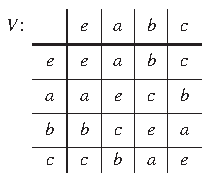
\includegraphics[width=\linewidth,height=.8\textheight,keepaspectratio]{assets/p070_09.pdf}\end{center}\end{minipage}
\end{center}
\end{BookFloat}

It is often useful to draw a\textit{ subgroup diagram} of the subgroups of a group. In such a diagram, a line running downward from a group \BookInline{G} to a group \BookInline{H} means that \BookInline{H} is a subgroup of \BookInline{G.} Thus the larger group is placed nearer the top of the diagram. Figure 5.10 contains the subgroup diagrams for the groups \BookInline{\mathbb{Z}_{4}} and \BookInline{V} of Example 5.7.

\begin{BookFloat}{05_subgroups-p70-9}
\begin{center}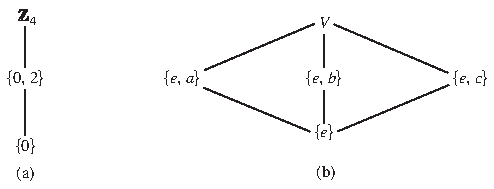
\includegraphics[width=0.677\linewidth,height=.8\textheight,keepaspectratio]{assets/p070_11.pdf}\end{center}
\begin{center}\small\textbf{5.10 Figure}\end{center}
\end{BookFloat}

(a) Subgroup diagram for \BookInline{\mathbb{Z}_{4}.(}b) Subgroup diagram for V.

Note that if \BookInline{H\leq G} and \BookInline{a\in H,\allowbreak } then by Theorem 2.17, the equation\textit{ ax} \BookInline{= a} must have a unique solution, namely the identity element of \BookInline{H.} But this equation can also 
% Source PDF page 71; original printed page 54
\BookSource{71}{54}
be viewed as one in \BookInline{G,\allowbreak } and we see that this unique solution must also be the identity element \BookInline{e} of \BookInline{G.} A similar argument then applied to the equation\textit{ ax} \BookInline{= e,\allowbreak } viewed in both \BookInline{H} and \BookInline{G,\allowbreak } shows that the inverse \BookInline{a^{- 1}} of \BookInline{a} in \BookInline{G} is also the inverse of \BookInline{a} in the subgroup \BookInline{H.}

\end{BookBody}

\BookNarrativetrue

\begin{BookBody}

\BookLabel{5.11 Example} Let \BookInline{F} be the group of all real-valued functions with domain \BookInline{\mathbb{R}} under addition. The subset of \BookInline{F} consisting of those functions that are continuous is a subgroup of \BookInline{F,\allowbreak } for the sum of continuous functions is continuous, the function \BookInline{f} where \BookInline{f(x)= 0} for all \BookInline{x} is continuous and is the additive identity element, and if \BookInline{f} is continuous, then \BookInline{- f} is continuous\BookInline{.}\BookEnd{\blacktriangle}

It is convenient to have routine steps for determining whether a subset of a group \BookInline{G} is a subgroup of \BookInline{G.} Example 5.11 indicates such a routine, and in the next theorem, we demonstrate carefully its validity.

\BookLabel{5.12 Theorem} A subset \BookInline{H} of a group \BookInline{G} is a subgroup of \BookInline{G} if and only if

\BookExercise{1.}{\BookInline{H} is closed under the binary operation of \BookInline{G,\allowbreak }}

\BookExercise{2.}{the identity element \BookInline{e} of \BookInline{G} is in \BookInline{H,\allowbreak } and}

\BookExercise{3.}{for all \BookInline{a\in H,\allowbreak a^{- 1}\in H} also.}

\BookLabel{\textit{Proof}} The fact that if \BookInline{H\leq G} then Conditions 1, 2, and 3 must hold follows at once from the definition of a subgroup and from the remarks preceding Example 5.11.

Conversely, suppose \BookInline{H} is a subset of a group \BookInline{G} such that Conditions 1, 2, and 3 hold. By 2 we have at once that \BookInline{\mathcal{G}_{2}} is satisfied. Also \BookInline{\mathcal{G}_{3}} is satisfied by 3. It remains to check the associative axiom\BookInline{,\allowbreak \mathcal{G}_{1}.} But surely for all \BookInline{a,\allowbreak b,\allowbreak c\in H} it is true that \BookInline{(ab)c= } \BookInline{a(bc)} in \BookInline{H,\allowbreak } for we may actually view this as an equation in \BookInline{G,\allowbreak } where the associative law holds. Hence \BookInline{H\leq G.}\BookEnd{\blacklozenge}

\BookLabel{5.13 Example} Let \BookInline{F} be as in Example 5.11. The subset of \BookInline{F} consisting of those functions that are differentiable is a subgroup of \BookInline{F,\allowbreak } for the sum of differentiable functions is differentiable, the constant function 0 is differentiable, and if \BookInline{f} is differentiable, then \BookInline{- f} is differentiable\BookInline{.}\BookEnd{\blacktriangle}

\BookLabel{5.14 Example} Recall from linear algebra that every square matrix \BookInline{A} has associated with it a number det\BookInline{(A)} called its determinant, and that \BookInline{A} is invertible if and only if det\BookInline{(A)\neq 0.} If \BookInline{A} and \BookInline{B} are square matrices of the same size, then it can be shown that det\BookInline{(AB)= } det\BookInline{(A)\cdot } det\BookInline{(B).} Let \BookInline{G} be the multiplicative group of all invertible \BookInline{n\times n} matrices with entries in \BookInline{\mathbb{C}} and let \BookInline{T} be the subset of \BookInline{G} consisting of those matrices with determinant 1. The equation det\BookInline{(AB)= } det\BookInline{(A)\cdot } det\BookInline{(B)} shows that \BookInline{T} is closed under matrix multiplication. Recall that the identity matrix \BookInline{I_{n}} has determinant 1. From the equation det\BookInline{(A)\cdot } det\BookInline{(A^{- 1})= } det\BookInline{(AA^{- 1})= } det\BookInline{(I_{n})= 1,\allowbreak } we see that if det\BookInline{(A)= 1,\allowbreak } then det\BookInline{(A^{- 1})= 1.} Theorem 5.12 then shows that \BookInline{T} is a subgroup of \BookInline{G.}\BookEnd{\blacktriangle} Theorem 5.15 provides an alternate way of checking that a subset of a group is a subgroup.

\BookLabel{5.15 Theorem} A nonempty subset \BookInline{H} of the group \BookInline{G} is a subgroup of \BookInline{G} if and only if for all \BookInline{a,\allowbreak b\in G,\allowbreak } \BookInline{ab^{- 1}\in G.}

\BookLabel{\textit{Proof}} We leave the proof as Exercise 51. \BookEnd{\blacklozenge}

\noindent On the surface Theorem 5.15 may seem simpler than Theorem 5.12 since we only need to show that \BookInline{H} is not empty and one other condition. In practice, it is usually just as efficient to use Theorem 5.12. On the other hand, Theorem 5.16 can often be used efficiently.

\end{BookBody}

% Source PDF page 72; original printed page 55
\BookSource{72}{55}
\BookNarrativetrue

\begin{BookBody}

\BookLabel{5.16 Theorem} Let \BookInline{H} be a finite nonempty subset of the group \BookInline{G.} Then \BookInline{H} is a subgroup of \BookInline{G} if and only if \BookInline{H} is closed under the operation of \BookInline{G.}

\BookLabel{\textit{Proof}} We leave the proof as Exercise 57. \BookEnd{\blacklozenge}

\BookLabel{5.17 Example} Recall that \BookInline{U_{n}= \{z\in \mathbb{C}\mid z^{n}= 1\}.} We could use Theorem 5.16 to verify that \BookInline{U_{n}} is a subgroup of \BookInline{C^{\ast }} by noting that \BookInline{U_{n}} has exactly \BookInline{n} elements, so \BookInline{U_{n}} is a finite nonempty subset of \BookInline{\mathbb{C}^{\ast }} and if \BookInline{z_{1},\allowbreak z_{2}\in U_{n},\allowbreak } then \BookInline{(z_{1}z_{2})^{n}= 1,\allowbreak } which implies that \BookInline{U_{n}} is closed under multiplication\BookInline{.}\BookEnd{\blacktriangle}

\BookLabel{5.18 Example} We verify that the subset \BookInline{H= \{\iota = \rho ^{0},\allowbreak \rho,\allowbreak \rho ^{2},\allowbreak...,\allowbreak \rho ^{n- 1}\}\subset D_{n}} is a subgroup of \BookInline{D_{n}.} By Theorem 5.16, we only need to check that \BookInline{H} is closed under the operation of \BookInline{D_{n}.} Let \BookInline{k,\allowbreak r\in \mathbb{Z}_{n}.} Then \BookInline{\rho ^{k}\rho ^{r}= \rho ^{k+ _{n}r}\in H.} Therefore \BookInline{H\leq D_{n}.}\BookEnd{\blacktriangle}

\BookTextHeading{\textbf{Cyclic Subgroups}  }

\noindent Let us see how large a subgroup \BookInline{H} of \BookInline{\mathbb{Z}_{12}} would have to be if it contains 3. It would have to contain the identity element 0 and \BookInline{3+ 3,\allowbreak } which is 6. Then it has to contain \BookInline{6+ 3,\allowbreak } which is 9. Note that the inverse of 3 is 9 and the inverse of 6 is 6. It is easily checked that \BookInline{H= \{0,\allowbreak 3,\allowbreak 6,\allowbreak 9\}} is a subgroup of \BookInline{\mathbb{Z}_{12},\allowbreak } and it is the smallest subgroup containing 3.

Let us imitate this reasoning in a general situation. As we remarked before, for a general argument we always use multiplicative notation. Let \BookInline{G} be a group and let \BookInline{a\in G.} A subgroup of \BookInline{G} containing \BookInline{a} must, by Theorem 5.12, contain \BookInline{a^{n},\allowbreak } the result of computing products of \BookInline{a} and itself for \BookInline{n} factors for every positive integer \BookInline{n.} These positive integral powers of \BookInline{a} do give a set closed under multiplication. It is possible, however, that the inverse of \BookInline{a} is not in this set. Of course, a subgroup containing \BookInline{a} must also contain \BookInline{a^{- 1},\allowbreak } and, in general, it must contain \BookInline{a^{- m}} for all \BookInline{m\in \mathbb{Z}^{+ }.} It must contain the identity element \BookInline{e= a^{0}.} Summarizing\BookInline{,\allowbreak a} \textit{subgroup of} \BookInline{G} \textit{containing the element} \BookInline{a} \textit{must} \textit{contain all elements} \BookInline{a^{n}(}\textit{or} \BookInline{na} \textit{for additive groups})\textit{ for all} \BookInline{n\in \mathbb{Z}.} That is, a subgroup containing \BookInline{a} must contain \BookInline{\{a^{n}\mid n\in \mathbb{Z}\}.} Observe that these powers \BookInline{a^{n}} of \BookInline{a} need not be distinct. For example, in the group \BookInline{V} of Example 5.7,

\begin{center}\begin{adjustbox}{max width=\linewidth}\BookInline{\displaystyle a^{2}= e,\allowbreak a^{3}= a,\allowbreak a^{4}= e,\allowbreak a^{- 1}= a,\allowbreak \;\text{and so on}\;.}\end{adjustbox}\end{center}

\noindent We have almost proved the next theorem.

\BookLabel{5.19 Theorem} Let \BookInline{G} be a group and let \BookInline{a\in G.} Then

\begin{center}\begin{adjustbox}{max width=\linewidth}\BookInline{\displaystyle H= \{a^{n}\mid n\in \mathbb{Z}\}}\end{adjustbox}\end{center}

\noindent is a subgroup of \BookInline{G} and is the smallest\label{bookfootnote:72:2:ref}\BookFootnote{2}{\label{bookfootnote:72:2:text}We may find occasion to distinguish between the terms\textit{ minimal} and\textit{ smallest} as applied to subsets of a set \BookInline{S} that have some property. A subset \BookInline{H} of \BookInline{S} is minimal with respect to the property if \BookInline{H} has the property, and no subset \BookInline{K\subset H,\allowbreak K\neq H,\allowbreak } has the property. If \BookInline{H} has the property and \BookInline{H\subseteq K} for every subset \BookInline{K} with the property, then \BookInline{H} is the smallest subset with the property. There may be many minimal subsets, but there can be only one smallest subset. To illustrate\BookInline{,\allowbreak \{e,\allowbreak a\},\allowbreak \{e,\allowbreak b\},\allowbreak } and \BookInline{\{e,\allowbreak c\}} are all minimal nontrivial subgroups of the group \BookInline{V.(}See Fig. 5.10.) However\BookInline{,\allowbreak V} contains no smallest nontrivial subgroup.} subgroup of \BookInline{G} that contains \BookInline{a,\allowbreak } that is, every subgroup containing \BookInline{a} contains \BookInline{H.}

\BookLabel{\textit{Proof}} We check the three conditions given in Theorem 5.12 for a subset of a group to give a subgroup. Since \BookInline{a^{r}a^{s}= a^{r+ s}} for \BookInline{r,\allowbreak s\in \mathbb{Z},\allowbreak } we see that the product in \BookInline{G} of two elements of \BookInline{H} is again in \BookInline{H.} Thus \BookInline{H} is closed under the group operation of \BookInline{G.} Also \BookInline{a^{0}= e,\allowbreak } so \BookInline{e\in H,\allowbreak } and for \BookInline{a^{r}\in H,\allowbreak a^{- r}\in H} and \BookInline{a^{- r}a^{r}= e.} Hence all the conditions are satisfied, and \BookInline{H\leq G.}

\end{BookBody}

% Source PDF page 73; original printed page 56
\BookSource{73}{56}
\BookNarrativetrue

\begin{BookBody}

Our arguments prior to the statement of the theorem showed that any subgroup of \BookInline{G} containing \BookInline{a} must contain \BookInline{H,\allowbreak } so \BookInline{H} is the smallest subgroup of \BookInline{G} containing \BookInline{a.}\BookEnd{\blacklozenge}

\BookLabel{5.20 Definition} Let \BookInline{G} be a group and let \BookInline{a\in G.} Then the subgroup \BookInline{\{a^{n}\mid n\in \mathbb{Z}\}} of \BookInline{G,\allowbreak } characterized in Theorem 5.19, is called the\textbf{ cyclic subgroup of} \BookInline{G} \textbf{generated by} \BookInline{a,\allowbreak } and denoted by \BookInline{\langle a\rangle.}\BookEnd{\blacksquare}

\BookLabel{5.21 Example} Let us find two of the cyclic subgroups to \BookInline{D_{10}.} We first consider \BookInline{\langle \mu \rho ^{k}\rangle } for \BookInline{k\in \mathbb{Z}_{10}.} Since \BookInline{(\mu \rho ^{k})^{2}= \iota } and \BookInline{(\mu \rho ^{k})^{- 1}= \mu \rho ^{k},\allowbreak } for any integer \BookInline{r,\allowbreak (\mu \rho ^{k})^{r}} is either \BookInline{\mu \rho ^{k}} or \BookInline{\iota.} Thus

\begin{center}\begin{adjustbox}{max width=\linewidth}\BookInline{\displaystyle \langle \mu \rho ^{k}\rangle = \{\iota ,\allowbreak \mu \rho ^{k}\}.}\end{adjustbox}\end{center}

\noindent Since \BookInline{\rho ^{- 1}= \rho ^{9},\allowbreak } every negative power of \BookInline{\rho } is also a positive power of \BookInline{\rho } and \BookInline{\rho ^{10}= \iota,\allowbreak }

\begin{center}\begin{adjustbox}{max width=\linewidth}\BookInline{\displaystyle \langle \rho \rangle = \{\iota ,\allowbreak \rho ,\allowbreak \rho ^{2},\allowbreak ...,\allowbreak \rho ^{9}\}.}\end{adjustbox}\end{center} \BookEnd{\blacktriangle}

\BookLabel{5.22 Definition} An element \BookInline{a} of a group \BookInline{G} \textbf{generates} \BookInline{G} and is a\textbf{ generator for} \BookInline{G} if \BookInline{\langle a\rangle = G.} A group \BookInline{G} is\textbf{ cyclic} if there is some element \BookInline{a} in \BookInline{G} that generates \BookInline{G.}\BookEnd{\blacksquare}

\BookLabel{5.23 Example} Let \BookInline{\mathbb{Z}_{4}} and \BookInline{V} be the groups of Example 5.7. Then \BookInline{\mathbb{Z}_{4}} is cyclic and both 1 and 3 are generators, that is,

\begin{center}\begin{adjustbox}{max width=\linewidth}\BookInline{\displaystyle \langle 1\rangle = \langle 3\rangle = \mathbb{Z}_{4}.}\end{adjustbox}\end{center}

\noindent However\BookInline{,\allowbreak V} is\textit{ not} cyclic, for \BookInline{\langle a\rangle,\allowbreak \langle b\rangle,\allowbreak } and \BookInline{\langle c\rangle } are proper subgroups of two elements. Of course\BookInline{,\allowbreak \langle e\rangle } is the trivial subgroup of one element\BookInline{.}\BookEnd{\blacktriangle}

\BookLabel{5.24 Example} The group \BookInline{\mathbb{Z}} under addition is a cyclic group. Both 1 and \BookInline{- 1} are generators for this group, and they are the only generators. Also, for \BookInline{n\in \mathbb{Z}^{+ },\allowbreak } the group \BookInline{\mathbb{Z}_{n}} under addition modulo \BookInline{n} is cyclic. If \BookInline{n>1,\allowbreak } then both 1 and \BookInline{n- 1} are generators, but there may be others\BookInline{.}\BookEnd{\blacktriangle}

\BookLabel{5.25 Example} Consider the group \BookInline{\mathbb{Z}} under addition. Let us find \BookInline{\langle 3\rangle.} Here the notation is additive, and \BookInline{\langle 3\rangle } must contain

\begin{center}\begin{adjustbox}{max width=\linewidth}\BookInline{\displaystyle \begin{aligned}3,\allowbreak 3+ 3&= 6,\allowbreak 3+ 3+ 3= 9,\allowbreak \;\text{and so on}\;,\allowbreak  \\ 0,\allowbreak - 3,\allowbreak - 3+ - 3&= - 6,\allowbreak - 3+ - 3+ - 3= - 9,\allowbreak \;\text{and so on}\;.\end{aligned}}\end{adjustbox}\end{center}

\noindent In other words, the cyclic subgroup generated by 3 consists of all multiples of 3, positive, negative, and zero. We denote this subgroup by \BookInline{3\mathbb{Z}} as well as \BookInline{\langle 3\rangle.} In a similar way, we shall let \BookInline{n\mathbb{Z}} be the cyclic subgroup \BookInline{\langle n\rangle } of \BookInline{\mathbb{Z}.} Note that \BookInline{6\mathbb{Z}<3\mathbb{Z}.}\BookEnd{\blacktriangle}

\BookLabel{5.26 Example} For each positive integer \BookInline{n,\allowbreak U_{n}} is the multiplicative group of the \BookInline{n}th roots of unity in \BookInline{\mathbb{C}.} These elements of \BookInline{U_{n}} can be represented geometrically by equally spaced points on a circle about the origin, as illustrated in Fig. 5.27. The point labeled represents the number

\begin{center}\begin{adjustbox}{max width=\linewidth}\BookInline{\displaystyle \zeta = \cos { \frac { 2 \pi } { n } } + i \sin { \frac { 2 \pi } { n } } .}\end{adjustbox}\end{center}

\noindent The geometric interpretation of multiplication of complex numbers, explained in Section 3, shows at once that as \BookInline{\zeta } is raised to powers, it works its way counterclockwise around the circle, landing on each of the elements of \BookInline{U_{n}} in turn. Thus \BookInline{U_{n}} under multiplication is a cyclic group, and \BookInline{\zeta } is a generator. The group \BookInline{U_{n}} is the cyclic subgroup \BookInline{\langle \zeta \rangle } of the group \BookInline{U} of all complex numbers \BookInline{z,\allowbreak } where \BookInline{|z|= 1,\allowbreak } under multiplication\BookInline{.}\BookEnd{\blacktriangle}

\end{BookBody}

% Source PDF page 74; original printed page 57
\BookSource{74}{57}
\BookNarrativefalse

\begin{BookBody}

\begin{BookFloat}{05_subgroups-p74-0}
\begin{center}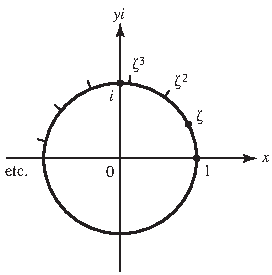
\includegraphics[width=0.373\linewidth,height=.8\textheight,keepaspectratio]{assets/p074_00.pdf}\end{center}
\begin{center}\small\textbf{5.27 Figure}\end{center}
\end{BookFloat}

\BookExerciseTitle{5}

\BookTextHeading{\textbf{Computations}}

\noindent In Exercises 1 through 6, determine whether the given subset of the complex numbers is a subgroup of the group \BookInline{\mathbb{C}} of complex numbers under addition.

\BookExercise{1.}{\BookInline{\mathbb{R}}}

\BookExercise{2.}{\BookInline{\mathbb{Q}^{+ }}}

\BookExercise{3.}{\BookInline{7\mathbb{Z}}}

\BookExercise{4.}{The set \BookInline{i\mathbb{R}} of pure imaginary numbers including 0}

\BookExercise{5.}{The set \BookInline{\pi \mathbb{Q}} of rational multiples of \BookInline{\pi }}

\BookExercise{6.}{The set \BookInline{\{\pi ^{n}\mid n\in \mathbb{Z}\}}}

\BookExercise{7.}{Which of the sets in Exercises 1 through 6 are subgroups of the group \BookInline{\mathbb{C}^{\ast }} of nonzero complex numbers under multiplication?}

\noindent In Exercises 8 through 13, determine whether the given set of invertible \BookInline{n\times n} matrices with real number entries is a subgroup of\textit{ GL}\BookInline{(n,\allowbreak \mathbb{R}).}

\BookExercise{8.}{The \BookInline{n\times n} matrices with determinant greater than or equal to 1}

\BookExercise{9.}{The diagonal \BookInline{n\times n} matrices with no zeros on the diagonal}

\BookExercise{10.}{The \BookInline{n\times n} matrices with determinant \BookInline{2^{k}} for some integer \BookInline{k}}

\BookExercise{11.}{The \BookInline{n\times n} matrices with determinant \BookInline{- 1}}

\BookExercise{12.}{The \BookInline{n\times n} matrices with determinant \BookInline{- 1} or 1}

\BookExercise{13.}{The set of all \BookInline{n\times n} matrices \BookInline{A} such that \BookInline{(A^{T})A= I_{n}.[}These matrices are called\textbf{ orthogonal.} Recall that \BookInline{A^{T},\allowbreak } the\textit{ transpose} of \BookInline{A,\allowbreak } is the matrix whose \BookInline{j}th column is the \BookInline{j}th row of \BookInline{A} for \BookInline{1\leq j\leq n,\allowbreak } and that the transpose operation has the property \BookInline{(AB)^{T}= (B^{T})(A^{T}).]}}

\noindent Let \BookInline{F} be the set of all real-valued functions with domain \BookInline{\mathbb{R}} and let \BookInline{\tilde { F }} be the subset of \BookInline{F} consisting of those functions that have a nonzero value at every point in \BookInline{\mathbb{R}.} In Exercises 14 through 19, determine whether the given subset of \BookInline{F} with the induced operation is (a) a subgroup of the group \BookInline{F} under addition, (b) a subgroup of the group \BookInline{\tilde { F }} under multiplication.

\BookExercise{14.}{The subset \BookInline{\tilde { F }}}

\BookExercise{15.}{The subset of all \BookInline{f\in F} such that \BookInline{f(1)= 0}}

\BookExercise{16.}{The subset of all \BookInline{f \in \tilde { F }} such that \BookInline{f(1)= 1}}

\BookExercise{17.}{The subset of all \BookInline{f \in \tilde { F }} such that \BookInline{f(0)= 1}}

\BookExercise{18.}{The subset of all \BookInline{f \in \tilde { F }} such that \BookInline{f(0)= - 1}}

\BookExercise{19.}{The subset of all constant functions in \BookInline{F.}}

\end{BookBody}

% Source PDF page 75; original printed page 58
\BookSource{75}{58}
\BookNarrativefalse

\begin{BookBody}

\BookExercise{20.}{Nine groups are given below. Give a\textit{ complete} list of all subgroup relations, of the form \BookInline{G_{i}\leq G_{j},\allowbreak } that exist between these given groups \BookInline{G_{1},\allowbreak G_{2},\allowbreak \cdots,\allowbreak G_{9}.} \BookInline{G_{1}= \mathbb{Z}} under addition \BookInline{G_{2}= 12\mathbb{Z}} under addition \BookInline{G_{3}= \mathbb{Q}^{+ }} under multiplication \BookInline{G_{4}= \mathbb{R}} under addition \BookInline{G_{5}= \mathbb{R}^{+ }} under multiplication \BookInline{G_{6}= \{\pi ^{n}\mid n\in \mathbb{Z}\}} under multiplication \BookInline{G_{7}= 3\mathbb{Z}} under addition \BookInline{G_{8}= } the set of all integral multiples of 6 under addition \BookInline{G_{9}= \{6^{n}\mid n\in \mathbb{Z}\}} under multiplication}

\BookExercise{21.}{Write at least 5 elements of each of the following cyclic groups. \textbf{a}\BookInline{.25\mathbb{Z}} under addition \textbf{b}\BookInline{.\{(\frac{1}{2})^{n}\mid n\in \mathbb{Z}\}} under multiplication \textbf{c}\BookInline{.\{\pi ^{n}\mid n\in \mathbb{Z}\}} under multiplication \textbf{d}\BookInline{.\langle \rho ^{3}\rangle } in the group \BookInline{D_{18}} \textbf{e}\BookInline{.\langle (1,\allowbreak 2,\allowbreak 3)(5,\allowbreak 6)\rangle } in the group \BookInline{S_{6}}}

\noindent In Exercises 22 through 25, describe all the elements in the cyclic subgroup of\textit{ GL}\BookInline{(2,\allowbreak \mathbb{R})} generated by the given \BookInline{2\times 2} \BookInline{\Big[\Big]} matrix. \BookInline{\Big[\Big]} \BookInline{\Big[\Big]} \BookInline{\Big[\Big]}

\BookExercise{22.}{\BookInline{\begin{bmatrix} 0 & - 1 \\ - 1 & 0 \end{bmatrix}}}

\BookExercise{23.}{\BookInline{\begin{bmatrix} 1 & 1 \\ 0 & 1 \end{bmatrix}}}

\BookExercise{24.}{\BookInline{\begin{bmatrix} 3 & 0 \\ 0 & 2 \end{bmatrix}}}

\BookExercise{25.}{\BookInline{\begin{bmatrix} 0 & - 2 \\ - 2 & 0 \end{bmatrix}}}

\BookExercise{26.}{Which of the following groups are cyclic? For each cyclic group, list all the generators of the group.}

\begin{center}\begin{adjustbox}{max width=\linewidth}\BookInline{\displaystyle G_{1}= \langle \mathbb{Z},\allowbreak + \rangle G_{2}= \langle \mathbb{Q},\allowbreak + \rangle G_{3}= \langle \mathbb{Q}^{+ },\allowbreak \cdot \rangle G_{4}= \langle 6\mathbb{Z},\allowbreak + \rangle}\end{adjustbox}\end{center}

\BookInline{G_{5}= \{6^{n}\mid n\in \mathbb{Z}\}} under multiplication

\BookInline{G_{6}= \{a+ b\sqrt{2}\mid a,\allowbreak b\in \mathbb{Z}\}} under addition

\noindent In Exercises 27 through 35, find the order of the cyclic subgroup of the given group generated by the indicated element.

\BookExercise{27.}{The subgroup of \BookInline{\mathbb{Z}_{4}} generated by 3}

\BookExercise{28.}{The subgroup of \BookInline{V} generated by \BookInline{c(}see Table 5.9)}

\BookExercise{29.}{The subgroup of \BookInline{U_{6}} generated by cos \BookInline{\begin{array} { r } { \frac { 2 \pi } { 3 } + i \sin \frac { 2 \pi } { 3 } } \end{array}}}

\BookExercise{30.}{The subgroup of \BookInline{\mathbb{Z}_{10}} generated by 8}

\BookExercise{31.}{The subgroup of \BookInline{\mathbb{Z}_{16}} generated by 12}

\BookExercise{32.}{The subgroup of the symmetric group \BookInline{S_{8}} generated by (2, 4, 6, 9)(3, 5, 7)}

\BookExercise{33.}{The subgroup of the symmetric group \BookInline{S_{10}} generated by (1, 10)(2, 9)(3, 8)(4, 7)(5, 6)}

\BookExercise{34.}{The subgroup of the multiplicative group \BookInline{G} of invertible \BookInline{4\times 4} matrices generated by}

\begin{center}\begin{adjustbox}{max width=\linewidth}\BookInline{\displaystyle \begin{bmatrix} 0 & 0 & 0 & 1 \\ 0 & 0 & 1 & 0 \\ 1 & 0 & 0 & 0 \\ 0 & 1 & 0 & 0 \end{bmatrix}}\end{adjustbox}\end{center}

\BookExercise{35.}{The subgroup of the multiplicative group \BookInline{G} of invertible \BookInline{4\times 4} matrices generated by}

\begin{center}\begin{adjustbox}{max width=\linewidth}\BookInline{\displaystyle \begin{bmatrix} 0 & 1 & 0 & 0 \\ 0 & 0 & 0 & 1 \\ 0 & 0 & 1 & 0 \\ 1 & 0 & 0 & 0 \end{bmatrix}}\end{adjustbox}\end{center}

\BookExercise{36.}{\textbf{. a} Complete Table 5.28 to give the group \BookInline{\mathbb{Z}_{6}} of 6 elements.}

\BookExercise{b.}{Compute the subgroups \BookInline{\langle 0\rangle,\allowbreak \langle 1\rangle,\allowbreak \langle 2\rangle,\allowbreak \langle 3\rangle,\allowbreak \langle 4\rangle,\allowbreak } and \BookInline{\langle 5\rangle } of the group \BookInline{\mathbb{Z}_{6}} given in part (a).}

\end{BookBody}

% Source PDF page 76; original printed page 59
\BookSource{76}{59}
\BookNarrativefalse

\begin{BookBody}

\BookExercise{c.}{Which elements are generators for the group \BookInline{\mathbb{Z}_{6}} of part (a)?}

\BookExercise{d.}{Give the subgroup diagram for the part (b) subgroups of \BookInline{\mathbb{Z}_{6}.(}We will see later that these are all the subgroups of \BookInline{\mathbb{Z}_{6}.)}}

\begin{BookFloat}{05_subgroups-p76-2}
\begin{center}\small\textbf{5.28 Table}\end{center}
\begin{center}\begin{adjustbox}{max width=\linewidth}
\renewcommand{\arraystretch}{1.2}\setlength{\tabcolsep}{5pt}
\begin{tabular}{c|c|c|c|c|c|c}
\BookInline{\mathbb{Z}_{6}:+ } & 0 & 1 & 2 & 3 & 4 & 5\\\hline
0 & 0 & 1 & 2 & 3 & 4 & 5\\\hline
1 & 1 & 2 & 3 & 4 & 5 & 0\\\hline
2 & 2 &  &  &  &  & \\\hline
3 & 3 &  &  &  &  & \\\hline
4 & 4 &  &  &  &  & \\\hline
5 & 5 &  &  &  &  & \\
\end{tabular}
\end{adjustbox}\end{center}
\end{BookFloat}

\BookTextHeading{\textbf{Concepts}}

\noindent In Exercises 37 and 38, correct the definition of the italicized term without reference to the text, if correction is needed, so that it is in a form acceptable for publication.

\BookExercise{37.}{A\textit{ subgroup} of a group \BookInline{G} is a subset \BookInline{H} of \BookInline{G} that contains the identity element \BookInline{e} of \BookInline{G} and also contains the inverse of each of its elements.}

\BookExercise{38.}{A group \BookInline{G} is\textit{ cyclic} if and only if there exists \BookInline{a\in G} such that \BookInline{G= \{a^{n}\mid n\in \mathbb{Z}\}.}}

\BookExercise{39.}{Determine whether each of the following is true or false.}

\BookExercise{a.}{The associative law holds in every group.}

\BookExercise{b.}{There may be a group in which the cancellation law fails.}

\BookExercise{c.}{Every group is a subgroup of itself.}

\BookExercise{d.}{Every group has exactly two improper subgroups.}

\BookExercise{e.}{In every cyclic group, every element is a generator.}

\BookExercise{f.}{A cyclic group has a unique generator.}

\BookExercise{g.}{Every set of numbers that is a group under addition is also a group under multiplication.}

\BookExercise{h.}{A subgroup may be defined as a subset of a group.}

\BookExercise{i.}{\textbf{i}\BookInline{.\mathbb{Z}_{4}} is a cyclic group.}

\BookExercise{j.}{Every subset of every group is a subgroup under the induced operation.}

\BookExercise{k.}{For any \BookInline{n\geq 3,\allowbreak } the dihedral group \BookInline{D_{n}} has at least \BookInline{n+ 2} cyclic subgroups.}

\BookExercise{40.}{Show by means of an example that it is possible for the quadratic equation \BookInline{x^{2}= e} to have more than two solutions in some group \BookInline{G} with identity \BookInline{e.}}

\noindent In Exercises 41 through 44 let \BookInline{B} be a subset of \BookInline{A,\allowbreak } and let \BookInline{b} be a particular element of \BookInline{B.} Determine whether the given set is a subgroup of the symmetric group \BookInline{S_{A}} under the induced operation. Here \BookInline{\sigma [B]= \{\sigma (x)\mid x\in B\}.}

\BookExercise{41.}{\BookInline{\{\sigma \in S_{A}\mid \sigma (b)= b\}}}

\BookExercise{42.}{\BookInline{\{\sigma \in S_{A}\mid \sigma (b)\in B\}}}

\BookExercise{43.}{\BookInline{\{\sigma \in S_{A}\mid \sigma [B]\subseteq B\}}}

\BookExercise{44.}{\BookInline{\{\sigma \in S_{A}\mid \sigma [B]= B\}}}

\BookTextHeading{\textbf{Theory}}

\noindent In Exercises 45 and 46, let \BookInline{\phi:G\to G^{\prime }} be an isomorphism of a group \BookInline{\langle G,\allowbreak \ast \rangle } with a group \BookInline{\langle G^{\prime },\allowbreak \ast ^{\prime }\rangle.} Write out a proof to convince a skeptic of the intuitively clear statement.

\end{BookBody}

% Source PDF page 77; original printed page 60
\BookSource{77}{60}
\BookNarrativefalse

\begin{BookBody}

\BookExercise{45.}{If \BookInline{H} is a subgroup of \BookInline{G,\allowbreak } then \BookInline{\phi [H]= \{\phi (h)\mid h\in H\}} is a subgroup of \BookInline{G^{\prime }.} That is, an isomorphism carries subgroups into subgroups.}

\BookExercise{46.}{If there is an \BookInline{a\in G} such that \BookInline{\langle a\rangle = G,\allowbreak } then \BookInline{G^{\prime }} is cyclic.}

\BookExercise{47.}{Show that if \BookInline{H} and \BookInline{K} are subgroups of an abelian group \BookInline{G,\allowbreak } then}

\begin{center}\begin{adjustbox}{max width=\linewidth}\BookInline{\displaystyle \{hk\mid h\in H\;\text{and}\;k\in K\}}\end{adjustbox}\end{center}

is a subgroup of \BookInline{G.}

\BookExercise{48.}{Find an example of a group \BookInline{G} and two subgroups \BookInline{H} and \BookInline{K} such that the set in Exercise 47 is not a subgroup of \BookInline{G.}}

\BookExercise{49.}{Prove that for any integer \BookInline{n\geq 3,\allowbreak S_{n}} has a subgroup isomorphic with \BookInline{D_{n}.}}

\BookExercise{50.}{Find the flaw in the following argument: “Condition 2 of Theorem 5.12 is redundant, since it can be derived from 1 and 3, for let \BookInline{a\in H.} Then \BookInline{a^{- 1}\in H} by 3, and by \BookInline{1,\allowbreak aa^{- 1}= e} is an element of \BookInline{H,\allowbreak } proving 2.”}

\BookExercise{51.}{Prove Theorem 5.15.}

\BookExercise{52.}{Prove that if \BookInline{G} is a cyclic group and \BookInline{|G|\geq 3,\allowbreak } then \BookInline{G} has at least 2 generators.}

\BookExercise{53.}{Prove that if \BookInline{G} is an abelian group, written multiplicatively, with identity element \BookInline{e,\allowbreak } then all elements \BookInline{x} of \BookInline{G} satisfying the equation \BookInline{x^{2}= e} form a subgroup \BookInline{H} of \BookInline{G.}}

\BookExercise{54.}{Repeat Exercise 53 for the general situation of the set \BookInline{H} of all solutions \BookInline{x} of the equation \BookInline{x^{n}= e} for a fixed integer \BookInline{n\geq 1} in an abelian group \BookInline{G} with identity \BookInline{e.}}

\BookExercise{55.}{Find a counterexample to Exercise 53 if the assumption of abelian is dropped.}

\BookExercise{56.}{Show that if \BookInline{a\in G,\allowbreak } where \BookInline{G} is a finite group with identity \BookInline{e,\allowbreak } then there exists \BookInline{n\in \mathbb{Z}^{+ }} such that \BookInline{a^{n}= e.}}

\BookExercise{57.}{Prove Theorem 5.16.}

\BookExercise{58.}{Let \BookInline{G} be a group and let \BookInline{a} be one fixed element of \BookInline{G.} Show that}

\begin{center}\begin{adjustbox}{max width=\linewidth}\BookInline{\displaystyle H_{a}= \{x\in G\mid xa= ax\}}\end{adjustbox}\end{center}

is a subgroup of \BookInline{G.}

\BookExercise{59.}{Generalizing Exercise 58, let \BookInline{S} be any subset of a group \BookInline{G.}}

\BookExercise{a.}{Show that \BookInline{H_{S}= \{x\in G\mid xs= sx} for all \BookInline{s\in S\}} is a subgroup of \BookInline{G.}}

\BookExercise{b.}{In reference to part (a), the subgroup \BookInline{H_{G}} is the\textbf{ center of} \BookInline{G.} Show that \BookInline{H_{G}} is an abelian group.}

\BookExercise{60.}{Let \BookInline{H} be a subgroup of a group \BookInline{G.} For \BookInline{a,\allowbreak b\in G,\allowbreak } let \BookInline{a\sim b} if and only if \BookInline{ab^{- 1}\in H.} Show that \BookInline{\sim } is an equivalence relation on \BookInline{G.}}

\BookExercise{61.}{For sets \BookInline{H} and \BookInline{K,\allowbreak } we define the\textbf{ intersection} \BookInline{H\cap K} by}

\begin{center}\begin{adjustbox}{max width=\linewidth}\BookInline{\displaystyle H\cap K= \{x\mid x\in H\;\text{and}\;x\in K\}.}\end{adjustbox}\end{center}

Show that if \BookInline{H\leq G} and \BookInline{K\leq G,\allowbreak } then \BookInline{H\cap K\leq G.(}Remember\BookInline{:\leq } denotes “is a subgroup of,” not “is a subset of.”)

\BookExercise{62.}{Prove that every cyclic group is abelian.}

\BookExercise{63.}{Let \BookInline{G} be a group and let \BookInline{G_{n}= \{g^{n}\mid g\in G\}.} Under what hypothesis about \BookInline{G} can we show that \BookInline{G_{n}} is a subgroup of \BookInline{G}?}

\BookExercise{64.}{Show that a group with no proper nontrivial subgroups is cyclic.}

\BookExercise{65.}{Cracker Barrel Restaurants place a puzzle called “Jump All But One Game” at each table. The puzzle starts with golf tees arranged in a triangle as in Figure 5.29a where the presence of a tee is noted with a solid dot and the absence is noted with a hollow dot. A move can be made if a tee can jump over one adjacent tee and land on an empty space. When a move is made, the tee that is jumped over is removed. A possible first move is shown in Figure 5.29b. The goal is to have just one remaining tee. Use the Klein 4-group to show that no matter what sequence of (legal) moves you make, the last remaining tee cannot be in a bottom corner position.}

\end{BookBody}

% Continuation on source PDF page 78, preceding Section 6
\BookNarrativetrue

\begin{BookBody}

\begin{BookFloat}{05_subgroups-p78-0}
\begin{center}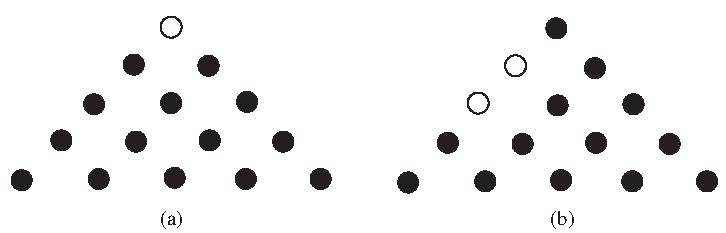
\includegraphics[width=0.995\linewidth,height=.8\textheight,keepaspectratio]{assets/p078_00.pdf}\end{center}
\begin{center}\small\textbf{5.29 Figure}\end{center}
\end{BookFloat}

\end{BookBody}
\ifdefined\BookMaster\let\BookFinish\relax\else\def\BookFinish{\end{document}}\fi\BookFinish
